\documentclass[a4paper,twoside]{article}
\usepackage[T1]{fontenc}
%\usepackage[encapsulated]{CJK}
\usepackage[utf8]{inputenc}
\usepackage{mathptmx}
\usepackage[scaled=0.9]{helvet}
\usepackage{courier}
\usepackage{pifont}
\usepackage{pdfpages}
\usepackage{fancyhdr}
%\usepackage{hyperref}
\usepackage{qrcode}
\usepackage[%
%  keepfiles,
  reusefiles
]{abcsvgintex}
\abcsvgauxdir{./abcsvgtmp/}
%\usepackage{ean13isbn}

\usepackage[top=2cm,bottom=2cm,left=1.5cm,right=1.5cm]{geometry}

\newcommand{\anneecopyright}{2014-2025}

%\renewcommand{\ocrb}{%
%%  \usefont{T1}{pcr}{m}{n}\fontsize{11pt}{11pt}\selectfont%
%%  \usefont{T1}{pcr}{b}{n}\fontsize{11pt}{11pt}\selectfont%
%  \usefont{T1}{phv}{m}{n}\fontsize{13pt}{11pt}\selectfont\X=1pt
%}
%\def\EANfinal{\testconsistence
%  \kern7\X\egroup
%  \hbox{\ocrbsmall \kern10\X \ISBNnum}\kern1\X
%  \dp0=0pt \box0 \kern1\X
%  \hbox{\ocrb\kern2\X\firstdigit\kern5\X \frontdigits\kern5\X \enddigits}
%  \egroup \global\barheight=0pt \gdef\ISBNnum{}}

\setlength{\parindent}{0pt}

\newcommand{\includerh}[3][0pt]{%
  \raisebox{#1}{\includegraphics[height=#2]{#3}}%
}
\makeatletter
\newcommand{\isodate}{%
  \the\year-\ifnum\the\month<10 0\fi\the\month-\ifnum\the\day<10 0\fi\the\day~
  \@tempcnta=\time
  \@tempcntb=\@tempcnta
  \divide\@tempcntb by 60
  \multiply\@tempcntb by 60
  \advance\@tempcnta by -\@tempcntb
  \divide\@tempcntb by 60
  \the\@tempcntb :\ifnum\the\@tempcnta < 10 0\fi\the\@tempcnta
}
\makeatother
\begin{document}
\pagestyle{empty}
\begin{titlepage}
  \newgeometry{nohead,nofoot,top=0.5cm,bottom=1cm,left=1cm,right=1cm}%
  \vspace*{\fill}%
  \hspace*{\fill}\fbox{\parbox[c][0.95\textheight][c]{0.95\textwidth}{%
    \vspace*{0pt plus 0.7 fill}
    \begin{center}
      \LARGE
      Jean-Sébastien Bach
      
      \bigskip
      
      \Huge
      Suites pour violoncelle
      
      \bigskip
      
      \Large
      BWV 1007-1012
      
      \bigskip
      Transcrites pour clarinette basse (Si~\(\flat\))

%      {\small en clef de sol octaviée et en clef de fa}

    \vspace*{0pt plus 0.3 fill}

%    \includegraphics{inc/BasseUtBuffet}
    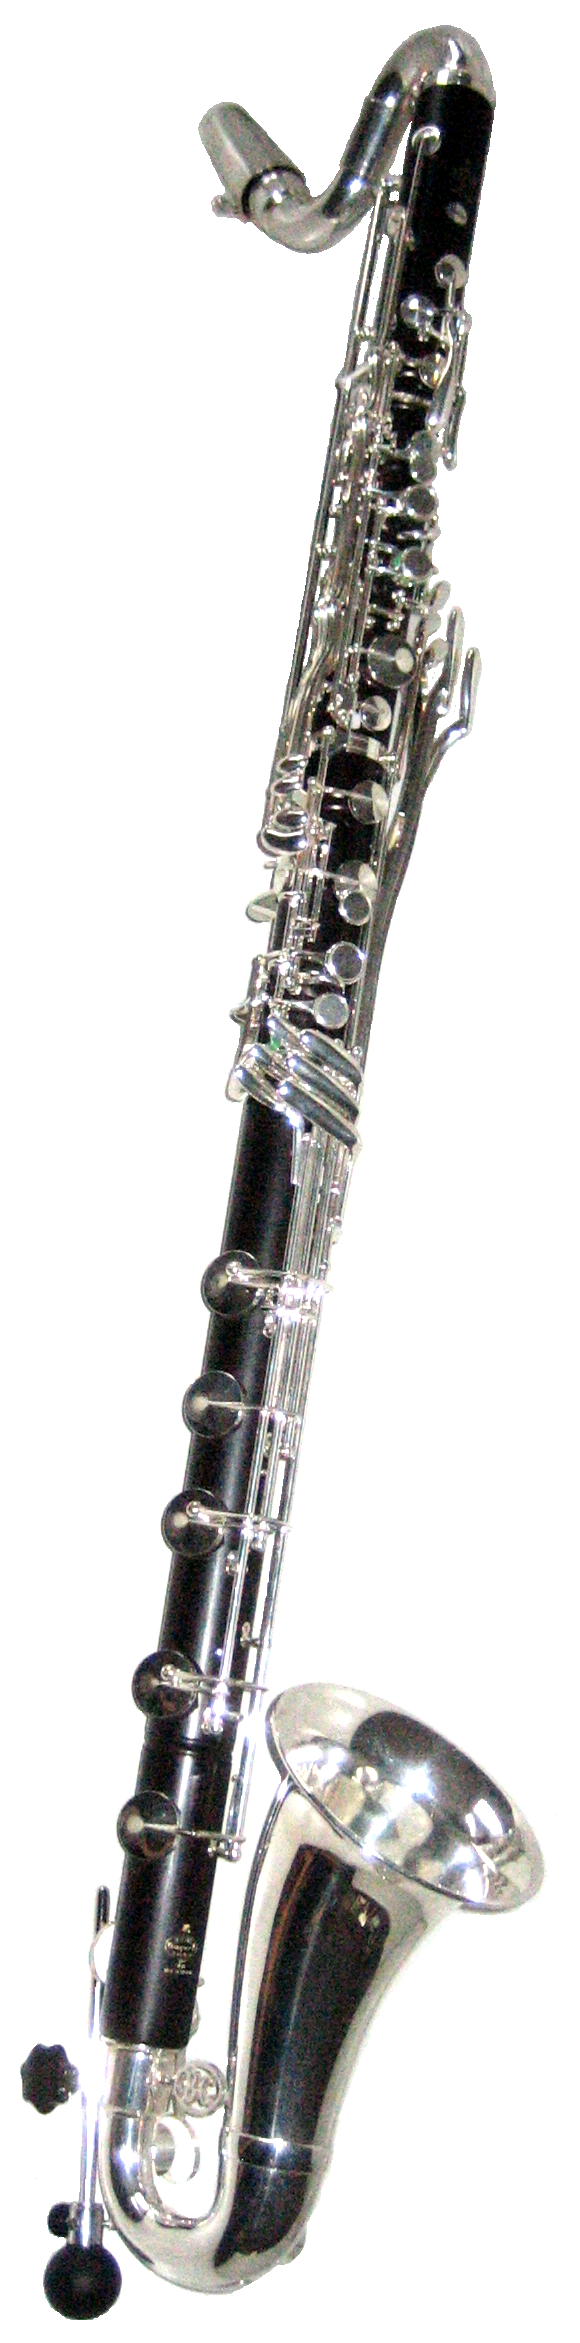
\includegraphics[scale=0.5]{inc/MaBasseBuffetUt_transp}
    
    \vspace*{0pt plus 0.5 fill}

    \normalsize\sffamily
    
    \copyright oclaribou editions \anneecopyright\quad frederic@oclaribou.fr
    
    https://www.oclaribou.fr/MusicBJS/BJSCelloSuites
        
    \bigskip
    
    \small
    http://creativecommons.org/licenses/by-sa/3.0/
    
    \smallskip
    
    
\includegraphics[width=2cm]{inc/by-sa}

    \end{center}
    \vspace*{0pt plus 0.1 fill}
  }}\hspace*{\fill}
  \vspace*{\fill}
\end{titlepage}
\restoregeometry

\cleardoublepage
%% page impaire
  \newgeometry{nohead,nofoot,top=0.5cm,bottom=1cm,left=1cm,right=1cm}%
   \vspace*{\fill}
%  \hspace*{\fill}\parbox[c][0.95\textheight][c]{0.95\textwidth}{%
    \begin{center}
      \LARGE
      Jean-Sébastien Bach
      
      \bigskip
      
      \Huge
      Suites pour violoncelle
      
      \bigskip
      
      \Large
      BWV 1007-1012
      
      \bigskip
      Transcrites pour clarinette basse (Si~\(\flat\))
      
  \vspace*{\fill}

  \hspace*{1.8cm}\parbox{0.7\textwidth}{%
    \large
	Transcriptions établies d'après les documents suivants~:
	\quad\begin{quote}
	\begin{itemize}
	  \item[\textbf{07437}] manuscrit attribué à Anna Magdalena Bach~;

	  \item[\textbf{12165}] édité par Alfred Dörffel, publié par Breitkopf \& Härtel en 1879~;

	  \item[\textbf{75794}] manuscrit attribué à Johann Peter Kellner.
	\end{itemize}
	\end{quote}
	disponibles sur la «~Petrucci Music Library~» IMSLP (\textsf{https://imslp.org/}) \\
	sous les références indiquées.
  }

%\vspace{5cm}
%\textsf{\normalsize ISBN 978-1-291-69214-3}

    \end{center}
%  }\hspace*{\fill}
  
  
  \vspace*{\fill}

\newpage
\restoregeometry

\mbox{}\newpage

\pagestyle{fancy}
\fancyfoot[C]{\thepage}
%\fancyfoot[OR]{\sffamily\small Source~: IMSLP 12165, 07437 et 75794\ \includerh[-0.2\totalheight]{2ex}{inc/by-sa_small}}
%\fancyfoot[EL]{\includerh[-0.2\totalheight]{2ex}{inc/by-sa_small}\ \sffamily\small Source~: IMSLP 12165, 07437 et 75794}
\fancyfoot[OR]{\includerh[-0.2\totalheight]{2ex}{inc/by-sa_small}}
\fancyfoot[EL]{\includerh[-0.2\totalheight]{2ex}{inc/by-sa_small}}
\fancyfoot[OL,ER]{\sffamily\copyright oclaribou editions \anneecopyright}
%\fancyhead[OR,EL]{Suites pour violoncelle BWV 1007-1012 (clarinette basse)}
\fancyhead[OR,EL]{}
\fancyhead[OL,ER]{}
\renewcommand{\headrulewidth}{0pt}

%% Table of contents
%\vspace*{1cm}
\begin{center}
{\LARGE Table des matières}

\vspace{1cm}
\large
\newlength{\titlelen}
\settowidth{\titlelen}{Allemande}
\addtolength{\titlelen}{0.5em}
\newlength{\titleseplen}
\setlength{\titleseplen}{0.1cm}
\newlength{\suitesep}
\setlength{\suitesep}{1cm}
\abcsvgsettings{%
  raise=-0.5\height+0.5ex,
}%
\abcsvgpdfsettings{%
	pagewidth=13cm,
	linebreak=\string$, linebreak=\string$,
	maxshrink=1.0,
	scale=0.5,
	measurenb=-1,
	writefields=Q 0,
	stretchlast=1
}%
%\abcsvgrebuildnext
\begin{itemize}
  \item \textbf{Suite n°I BWV 1007 en Sol majeur (La majeur)} \dotfill\ \pageref{SuiteI}
  \begin{enumerate}
	\item \makebox[\titlelen][l]{Prélude}
\begin{abcsvg}
  M:4/4
  L:1/16
  K:Amaj clef=treble-8 octave=1 transpose=10
  (A,,E,C)B, CE,CE, (A,,E,C)B, CE,CE, |
  (A,,F,D)C DF,DF, (A,,F,D)C DF,DF, |
\end{abcsvg}
  \makebox[2cm][l]{ \dotfill\ \pageref{Iprelude}}
  \par\vspace{\titleseplen}

	\item \makebox[\titlelen][l]{Allemande}
\begin{abcsvg}
  M:4/4
  L:1/16
  K:Amaj clef=treble_8
  C |
  {A,,E,}C4- C(B,A,G,) (A,E,F,G,) (A,B,CD) |
  (ECA,G,) (A,F,E,D,) (C,D,E,F,) (G,A,B,C) |
\end{abcsvg}
  \makebox[2cm][l]{ \dotfill\ \pageref{Iallemande}}
  \par\vspace{\titleseplen}

	\item \makebox[\titlelen][l]{Courante}
\begin{abcsvg}
  M:3/4
  L:1/16
  K:Amaj clef=treble_8
  A,2 |
  A,2E,2 A,,2(CD EDCB,) |
  C2E,2 A,,2(A,B, C2)A,2 |
  F,2D,2 D,,2(B,C DCB,A,) |
\end{abcsvg}
  \makebox[2cm][l]{ \dotfill\ \pageref{Icourante}}
  \par\vspace{\titleseplen}

	\item \makebox[\titlelen][l]{Sarabande}
\begin{abcsvg}
  M:3/4
  L:1/8
  K:Amaj clef=treble_8
  {A,,E,}C2 ({A,,F,}D3 C) |
  (G,/2B,/2C/2)D/2 {A,,E,}!trill!C2 (B,A,) |
  E=G, (F,3/2(3E,/4D,/4C,/4 D,)F, |
\end{abcsvg}
  \makebox[2cm][l]{ \dotfill\ \pageref{Isarabande}}
  \par\vspace{\titleseplen}

	\item \makebox[\titlelen][l]{Menuets}
\begin{abcsvg}
  M:3/4
  L:1/8
  K:Amaj clef=treble_8
  P:Menuet I
  (A,,E, C2) (B,C/2D/2) |
  (CB,)(A,G,)(A,E,) |
  (F,A,)(DB,)(G,E) |
  TC4 B,2 |
\end{abcsvg}
  \\
  \hspace*{\titlelen}
\begin{abcsvg}
  M:3/4
  L:1/8
  K:Em clef=treble_8
  P:Menuet II
  |: (=CB,C)E,=F,A,, |
  =G,,2 B,2 E,2 |
  (A,^G,A,)=C,D,=F,, |
  (E,,B,,E,)A,^G,B, |
\end{abcsvg}
  \makebox[2cm][l]{ \dotfill\ \pageref{Imenuets}}
  \par\vspace{\titleseplen}

	\item \makebox[\titlelen][l]{Gigue}
\begin{abcsvg}
  M:6/8
  L:1/8
  K:Amaj clef=treble_8
  E, |
  A,(E,F,) F,(D,E,) |
  E,A,E, C,A,,E, |
  (A,/2B,/2C)B, (B,/2C/2D)C |
  {A,,E,}!trill!C3 {E,}B,2 B, |
\end{abcsvg}
  \makebox[2cm][l]{ \dotfill\ \pageref{Igigue}}
  \end{enumerate}
  \par\vspace{\suitesep}

  \item \textbf{Suite n°II BWV 1008 en Ré mineur (Mi mineur)} \dotfill\ \pageref{SuiteII}
  \begin{enumerate}
  \item \makebox[\titlelen][l]{Prélude}
\begin{abcsvg}
  M:3/4
  L:1/16
  K:Em clef=treble_8
  E,2G,2 B,4- B,(G,F,E,) |
  (^D,F,A,B,) C4- C(B,A,G,) |
  (F,A,C^D) F3C (B,A,G,F,) |
\end{abcsvg}
  \makebox[2cm][l]{ \dotfill\ \pageref{IIprelude}}
  \par\vspace{\titleseplen}

  \item \makebox[\titlelen][l]{Allemande}
\begin{abcsvg}
  M:C
  L:1/16
  K:Em clef=treble_8
  B,|{E,,B,,G,}B,2(CB,) (A,G,)(F,E,) (E,^D,)(E,F,) B,,2C,A,, |
  G,,B,,E,G,, F,,2^D,2 {E,,B,,}E,3F, G,A,B,C |
\end{abcsvg}
  \makebox[2cm][l]{ \dotfill\ \pageref{IIallemande}}
  \par\vspace{\titleseplen}

  \item \makebox[\titlelen][l]{Courante}
\begin{abcsvg}
  M:3/4
  L:1/16
  K:Em clef=treble_8
  E | EB,G,B, E,G,A,B, CB,CA, |
  {B,}^D,4- D,E,F,G, A,G,A,F, |
\end{abcsvg}
  \makebox[2cm][l]{ \dotfill\ \pageref{IIcourante}}
  \par\vspace{\titleseplen}

  \item \makebox[\titlelen][l]{Sarabande}
\begin{abcsvg}
  M:3/4
  L:1/16
  K:Em clef=treble_8
  E,3F, {B,,}!trill!F,6 E,F, |
  {E,,B,,}G,6 F,2E,2D,2 |
  C,2A,2 !parupmordent!G,2(F,G, A,B,CE,)|
  !trill!^D,6 ^C,2B,,2A,,2 |
\end{abcsvg}
  \makebox[2cm][l]{ \dotfill\ \pageref{IIsarabande}}
  \par\vspace{\titleseplen}

  \item \makebox[\titlelen][l]{Menuets}
\begin{abcsvg}
  M:3/4
  L:1/8
  K:Em clef=treble_8
  [P:Menuet I]
  {E,G,}B,4 C2 |
  {D,F,}(CB,)CA, B,2 |
  {C,}E,2 A,2 G,F, |
  {B,,}(G,F,E,)^D,^C,B,, |
\end{abcsvg}
  \\
  \hspace*{\titlelen}
\begin{abcsvg}
  K:Emaj clef=treble_8
  [P:Menuet II]
  |: !trill!G,2 E,F,G,A, |
  B,2 G,,2 B,2 |
  (A,,C,) F,2 A,2 |
  (E,D,C,D,B,,A,,) |
\end{abcsvg}
  \makebox[2cm][l]{ \dotfill\ \pageref{IImenuets}}
  \par\vspace{\titleseplen}

  \item \makebox[\titlelen][l]{Gigue}
\begin{abcsvg}
  M:3/8
  L:1/16
  K:Em clef=treble_8
  B,2 | E,4 C2 |
  ^D,4 A,2 |
  G,F,G,A,B,2 |
  E,4 E2 |
  (F,G,A,2)C2 |
  (D,E,F,2)D2 |
\end{abcsvg}
  \makebox[2cm][l]{ \dotfill\ \pageref{IIgigue}}
  \end{enumerate}
  \newpage
  
  \item \textbf{Suite n°III BWV 1009 en Ut majeur (Ré majeur)} \dotfill\ \pageref{SuiteIII}
\begin{enumerate}
  \item \makebox[\titlelen][l]{Prélude}
\begin{abcsvg}
  M:3/4
  L:1/16
  K:D clef=treble_8
  D2CB, A,G,F,E, D,A,,F,,A,, |
  D,,4- D,,E,,F,,G,, A,,B,,C,D, |
  (E,D,C,B,,) (A,,B,,C,D,) (E,F,G,E,) |
\end{abcsvg}
  \makebox[2cm][l]{ \dotfill\ \pageref{IIIprelude}}
  \par\vspace{\titleseplen}

  \item \makebox[\titlelen][l]{Allemande}
\begin{abcsvg}
  M:C
  L:1/16
  K:D clef=treble_8
  xA,B,C | (DC/2B,/2A,)G, (F,A,/2G,/2F,)E, (D,A,,/2G,,/2F,,)E,, D,,D,E,F, |
\end{abcsvg}
  \makebox[2cm][l]{ \dotfill\ \pageref{IIIallemande}}
  \par\vspace{\titleseplen}

  \item \makebox[\titlelen][l]{Courante}
\begin{abcsvg}
  M:3/4
  L:1/8
  K:D clef=treble_8
  D | DA,F,D,A,,F,, |
  D,,(DEDCD) | 
  ECA,E,C,A,, |
  G,,(EDCB,A,) |
  D(CB,A,G,F,) |
\end{abcsvg}
  \makebox[2cm][l]{ \dotfill\ \pageref{IIIcourante}}
  \par\vspace{\titleseplen}

  \item \makebox[\titlelen][l]{Sarabande}
\begin{abcsvg}
  M:3/4
  L:1/16
  K:D clef=treble_8
  {D,,A,,F,}D4 {E,}D3B, C4 |
  {D,,A,,F,}=C4 {G,}C3A, B,4 |
  {^C,}E,2(F,G,) {D,,A,,}G,3E, F,2G,2 |
\end{abcsvg}
  \makebox[2cm][l]{ \dotfill\ \pageref{IIIsarabande}}
  \par\vspace{\titleseplen}

  \item \makebox[\titlelen][l]{Bourrées}
\begin{abcsvg}
  M:C|
  L:1/8
  K:D clef=treble_8
  P:Bourrée I
  F,G, |
  A,2 (D,C,) D,2 D2 |
  {A,,E,}C2 B,C A,2 E,F, |
  G,2 (C,B,,) C,2 A,2 |
  ({D,,A,,}G,F,E,F,) D,2 (DC) |
\end{abcsvg}
  \\
  \hspace*{\titlelen}
\begin{abcsvg}
  M:C|
  L:1/8
  K:Am clef=treble_8
  P:Bourrée II
  |: DE |
  F2 ED ^C2 D2 |
  (ED^CB,) (A,G,F,E,) |
  F,(A,G,F,) E,(G,F,E,) |
\end{abcsvg}
  \makebox[2cm][l]{ \dotfill\ \pageref{IIIbourrees}}
  \par\vspace{\titleseplen}

  \item \makebox[\titlelen][l]{Gigue}
\begin{abcsvg}
  M:3/8
  L:1/16
  K:Dmaj clef=treble_8
  A,2 | D2(D,E,F,G,) |
  (A,2B,2)C2 |
  (D2A,2)F2 |
  (D2A,2)F2 |
  (EDEF)G2 |
  (C2D2)F,2 |
  (A,,2E,2)D2 |
  (C2A,2)E2 |
\end{abcsvg}
  \makebox[2cm][l]{ \dotfill\ \pageref{IIIgigue}}
  \end{enumerate}
  \par\vspace{\suitesep}
  
  \item \textbf{Suite n°IV BWV 1010 en Mi\,\(\flat\) majeur (Fa majeur)} \dotfill\ \pageref{SuiteIV}
\begin{enumerate}
  \item \makebox[\titlelen][l]{Prélude}
\begin{abcsvg}
  M:C|
  L:1/8
  K:Fmaj clef=treble_8
  F,,FCA, CF,A,C, |
  F,,FCA, CF,A,C, |
  F,,_ECA, CF,A,C, |
  F,,_ECA, CF,A,C, |
\end{abcsvg}
  \makebox[2cm][l]{ \dotfill\ \pageref{IVprelude}}
  \par\vspace{\titleseplen}

  \item \makebox[\titlelen][l]{Allemande}
\begin{abcsvg}
  M:C
  L:1/16
  K:Fmaj clef=treble_8
  C2 | (F2ED) CB,A,B, CB,A,G, F,E,D,C, |
  (D,F,G,A,) (B,A,G,F,) (E,F,G,E,) !trill!C,2B,,2 |
\end{abcsvg}
  \makebox[2cm][l]{ \dotfill\ \pageref{IVallemande}}
  \par\vspace{\titleseplen}

  \item \makebox[\titlelen][l]{Courante}
\begin{abcsvg}
  M:3/4
  L:1/8
  K:Fmaj clef=treble_8
  F, | F,C,D,B,,G,,E, |
  F,2 F,,/2E,/2F,/2G,/2 A,/2G,/2A,/2=B,/2 |
  CG,A,F,D,=B, |
  C2 C,(!trill!_B,,A,,)F, |
\end{abcsvg}
  \makebox[2cm][l]{ \dotfill\ \pageref{IVcourante}}
  \par\vspace{\titleseplen}

  \item \makebox[\titlelen][l]{Sarabande}
\begin{abcsvg}
  M:3/4
  L:1/8
  K:Fmaj clef=treble_8
  {F,}C2 {F,}D2 {F,}_E2 |
  {B,,2F,2}_E3/2C/2 D2- D/2('C/2B,/2A,/2) |
  {C,}G,2 {C,}A,2 {C,}B,2 |
  {F,,2C,2}B,3/2G,/2 A,3/2C/2 F,2-' |
\end{abcsvg}
  \makebox[2cm][l]{ \dotfill\ \pageref{IVsarabande}}
  \par\vspace{\titleseplen}

  \item \makebox[\titlelen][l]{Bourrées}
\begin{abcsvg}
  M:C|
  L:1/8
  K:Fmaj clef=treble_8
  P:Bourrée I
  (F,/2G,/2A,/2B,/2 | C2) DB, C2 DA, |
  B,2 G,2 G,,2 (E,/2F,/2G,/2A,/2 |
  B,2) CA, B,2 CG, |
\end{abcsvg}
  \\
  \hspace*{\titlelen}
\begin{abcsvg}
  M:C|
  L:1/8
  K:Fmaj clef=treble_8
  P:Bourrée II
  [| {A,,}F,2 |
  {B,,}F,2 G,2-' {C,}G,2 E,2 |
  {D,}F,G, A,2-' {A,,}A,2 F,2 |
  B,,2 G,2 C,2 E,2 |
\end{abcsvg}
  \makebox[2cm][l]{ \dotfill\ \pageref{IVbourrees}}
  \par\vspace{\titleseplen}

  \item \makebox[\titlelen][l]{Gigue}
\begin{abcsvg}
  M:12/8
  L:1/8
  K:Fmaj clef=treble_8
  F, | (F,E,F,) (C,D,E,) (F,E,F,) (A,G,A,) |
  (F,E,F,) (C,D,E,) F,,3- F,,2 A, |
  (G,F,G,) (CA,B,) (A,G,A,) (F,G,A,) |
\end{abcsvg}
  \makebox[2cm][l]{ \dotfill\ \pageref{IVgigue}}
  \end{enumerate}
  \newpage
  
  \item \textbf{Suite n°V BWV 1011 en Ut mineur (Ré mineur)} \dotfill\ \pageref{SuiteV}
\begin{enumerate}
  \item \makebox[\titlelen][l]{Prélude}
\begin{abcsvg}
  M:C
  L:1/16
  K:Fmaj clef=treble_8
  {D,,}D,4- D,(A,,=B,,^C, D,E,F,G, F,E,F,D,) |
  {D,,^C,G,}B,6 B,2 (A,2B,G,) (F,2G,E,) |
  {D,}F,4 D,,4 D,4- D,D,E,F, |
\end{abcsvg}
  \makebox[2cm][l]{ \dotfill\ \pageref{Vprelude}}
  \par\vspace{\titleseplen}

  \item \makebox[\titlelen][l]{Allemande}
\begin{abcsvg}
  M:C
  L:1/16
  K:Fmaj clef=treble_8
  D2 | {D,,A,,F,}D4- D(CB,A,) B,3G, {^C,}A,3E, |
  ({D,}F,4 D,)C,B,,A,, B,,3G,, A,,3E, |
  {F,,A,,}E,3D,/2^C,/2 D,3A, B,,3A, (G,F,E,D,) |
\end{abcsvg}
  \makebox[2cm][l]{ \dotfill\ \pageref{Vallemande}}
  \par\vspace{\titleseplen}

  \item \makebox[\titlelen][l]{Courante}
\begin{abcsvg}
  M:3/2
  L:1/8
  K:Fmaj clef=treble_8
  D, | {D,,}D,3 E, (F,G,A,B,) (A,G,A,F,) |
  {E,,^C,}G,3 F, (F,E,D,^C,) D,3 E, |
  {D,,}A,,3 D,/2^C,/2 D,2 E,2 (G,F,E,D,) |
\end{abcsvg}
  \makebox[2cm][l]{ \dotfill\ \pageref{Vcourante}}
  \par\vspace{\titleseplen}

  \item \makebox[\titlelen][l]{Sarabande}
\begin{abcsvg}
  M:3/4
  L:1/8
  K:Fmaj clef=treble_8
  A,(F,^C,D,) B,,2 |
  D(B,^F,G,) ^C,2 |
  E(B,^F,G,) A,,A, |
  G,(F,^C,D,) D,,2 |
  (D,F,B,A,)(_ED) |
\end{abcsvg}
  \makebox[2cm][l]{ \dotfill\ \pageref{Vsarabande}}
  \par\vspace{\titleseplen}

  \item \makebox[\titlelen][l]{Gavottes}
\begin{abcsvg}
  M:C|
  L:1/8
  K:Fmaj clef=treble_8
  P:Gavotte I
  {D,F,}A,2 D2 | {G,}B,2 (CA,) {E,}B,2 (CG,) |
  A,2 (F,^C,) D,2 (B,F,) |
  G,2 (E,=B,,) (^C,E,) A,2 |
\end{abcsvg}
  \\
  \hspace*{\titlelen}
\begin{abcsvg}
  M:C|
  L:1/8
  K:Fmaj clef=treble_8
  P:Gavotte II
  |: (3A,G,A, (3_B,A,G, | A,2-(3A,G,F, (3E,F,G, (3F,E,D, |
  (3^C,D,E, (3A,,^C,E, (3A,G,A, (3_B,A,G, |
\end{abcsvg}
  \makebox[2cm][l]{ \dotfill\ \pageref{Vgavottes}}
  \par\vspace{\titleseplen}

  \item \makebox[\titlelen][l]{Gigue}
\begin{abcsvg}
  M:3/8
  L:1/8
  K:Dm clef=treble_8
  A, | F,>G,E, | F,>G,E, | D,3/2(C,/2B,,/2A,,/2) | B,,>D,A,, | G,,>F,D, | E,>F,D, | ^C,>E,A,, |
\end{abcsvg}
  \makebox[2cm][l]{ \dotfill\ \pageref{Vgigue}}
  \end{enumerate}
  \par\vspace{\suitesep}

  \item \textbf{Suite n°VI BWV 1012 en Ré majeur (Mi majeur)} \dotfill\ \pageref{SuiteVI}
\begin{enumerate}
  \item \makebox[\titlelen][l]{Prélude}
\begin{abcsvg}
  M:12/8
  L:1/8
  K:Emaj clef=treble_8
  !f!(E,E,)E, (E,E,)G, (E,E,)B, (E,E,)E |
  !p!(E,E,)E, (E,E,)G, (E,E,)B, (E,E,)E |
  !f!C(E,A,) (CDE) B,(E,G,) (B,DE) |
\end{abcsvg}
  \makebox[2cm][l]{ \dotfill\ \pageref{VIprelude}}
  \par\vspace{\titleseplen}

  \item \makebox[\titlelen][l]{Allemande}
\begin{abcsvg}
  M:C
  L:1/32
  K:Emaj clef=treble_8
  G2 | {E,B,}G8- G(FAG!beambr2!FEF/2D/2E) ({F,}E4!trill!D3E/2F/2) (EDCB,!beambr2!C/2D/2C/2D/2DC/2D/2)|
\end{abcsvg}
  \makebox[2cm][l]{ \dotfill\ \pageref{VIallemande}}
  \par\vspace{\titleseplen}

  \item \makebox[\titlelen][l]{Courante}
\begin{abcsvg}
  M:3/4
  L:1/8
  K:Emaj clef=treble_8
  E | E(E,/2F,/2G,)E,B,G, |
  EB,GEB=D |
  C(F/2G/2A)FcE |
  D(B,/2C/2D)B,FA, |
\end{abcsvg}
  \makebox[2cm][l]{ \dotfill\ \pageref{VIcourante}}
  \par\vspace{\titleseplen}

  \item \makebox[\titlelen][l]{Sarabande}
\begin{abcsvg}
  M:3/2
  L:1/4
  K:Emaj clef=treble_8
  {E,B,}G2 {B,}G3 A |
  ({A,,A,}F{A,}D) {G,}E3 c |
  ({B,,G,E}BG) {F,D}A3 B |
  ({E,B,}AG) (AF) G2 |
\end{abcsvg}
  \makebox[2cm][l]{ \dotfill\ \pageref{VIsarabande}}
  \par\vspace{\titleseplen}

  \item \makebox[\titlelen][l]{Gavottes}
\begin{abcsvg}
  M:C|
  L:1/8
  K:Emaj clef=treble_8
  P:Gavotte I
  {E,B,}G2 G2 |
  {A,,E,C}G2 FE {A,C}FG A2 |
  ({F,}EDCB,) {A,,F,D}B2 B2 |
\end{abcsvg}
  \\
  \hspace*{\titlelen}
\begin{abcsvg}
  M:C|
  L:1/8
  K:Emaj clef=treble_8
  P:Gavotte II
  |: {E,B,}GF G2 |
  B,2 {G,}B,2 {A,}C2 {F,}D2 |
  {E,}EDEF {E,,B,,G,}EF G2 |
\end{abcsvg}
  \makebox[2cm][l]{ \dotfill\ \pageref{VIgavottes}}
  \par\vspace{\titleseplen}

  \item \makebox[\titlelen][l]{Gigue}
\begin{abcsvg}
  M:6/8
  L:1/8
  K:Emaj clef=treble_8
  B | {G,}E3 {B,}FGA |
  {E,B,}GEB (B/2A/2G/2A/2B) |
  {G,}EB,E {B,}FGA |
  GEB, E,2 B |
\end{abcsvg}
  \makebox[2cm][l]{ \dotfill\ \pageref{VIgigue}}
  \end{enumerate}

\end{itemize}

\end{center}

\cleardoublepage
%% Suite n°I
\label{SuiteI}
\vspace*{2cm}

\begin{center}
\Large Suite n°I BWV 1007 en Sol majeur (La majeur)
\end{center}

\vspace{3cm}

\abcsvgsettings{%
  raise=-0.5\height+0.5ex,
}%
\abcsvgpdfsettings{%
	pagewidth=13cm,
	linebreak=\string$, linebreak=\string$,
	maxshrink=1.0,
	scale=0.5,
	measurenb=-1,
	writefields=Q 0,
	stretchlast=1
}%
\large
\settowidth{\titlelen}{Allemande}
\addtolength{\titlelen}{0.5em}
\setlength{\titleseplen}{1cm}
\begin{enumerate}
  \item \makebox[\titlelen][l]{Prélude}
\begin{abcsvg}
  M:4/4
  L:1/16
  K:Amaj clef=treble_8
  (A,,E,C)B, CE,CE, (A,,E,C)B, CE,CE, |
  (A,,F,D)C DF,DF, (A,,F,D)C DF,DF, |
\end{abcsvg}
\makebox[2cm][l]{ \dotfill\ \pageref{Iprelude}}
\par\vspace{\titleseplen}

  \item \makebox[\titlelen][l]{Allemande}
\begin{abcsvg}
  M:4/4
  L:1/16
  K:Amaj clef=treble_8
  C |
  {A,,E,}C4- C(B,A,G,) (A,E,F,G,) (A,B,CD) |
  (ECA,G,) (A,F,E,D,) (C,D,E,F,) (G,A,B,C) |
\end{abcsvg}
\makebox[2cm][l]{ \dotfill\ \pageref{Iallemande}}
\par\vspace{\titleseplen}

  \item \makebox[\titlelen][l]{Courante}
\begin{abcsvg}
  M:3/4
  L:1/16
  K:Amaj clef=treble_8
  A,2 |
  A,2E,2 A,,2(CD EDCB,) |
  C2E,2 A,,2(A,B, C2)A,2 |
  F,2D,2 D,,2(B,C DCB,A,) |
\end{abcsvg}
\makebox[2cm][l]{ \dotfill\ \pageref{Icourante}}
\par\vspace{\titleseplen}

  \item \makebox[\titlelen][l]{Sarabande}
\begin{abcsvg}
  M:3/4
  L:1/8
  K:Amaj clef=treble_8
  {A,,E,}C2 ({A,,F,}D3 C) |
  (G,/2B,/2C/2)D/2 {A,,E,}!trill!C2 (B,A,) |
  E=G, (F,3/2(3E,/4D,/4C,/4 D,)F, |
\end{abcsvg}
\makebox[2cm][l]{ \dotfill\ \pageref{Isarabande}}
\par\vspace{\titleseplen}

  \item \makebox[\titlelen][l]{Menuets}
\begin{abcsvg}
  M:3/4
  L:1/8
  K:Amaj clef=treble_8
  P:Menuet I
  (A,,E, C2) (B,C/2D/2) |
  (CB,)(A,G,)(A,E,) |
  (F,A,)(DB,)(G,E) |
  TC4 B,2 |
\end{abcsvg}
\\
\hspace*{\titlelen}
\begin{abcsvg}
  M:3/4
  L:1/8
  K:Em clef=treble_8
  P:Menuet II
  |: (=CB,C)E,=F,A,, |
  =G,,2 B,2 E,2 |
  (A,^G,A,)=C,D,=F,, |
  (E,,B,,E,)A,^G,B, |
\end{abcsvg}
\makebox[2cm][l]{ \dotfill\ \pageref{Imenuets}}
\par\vspace{\titleseplen}

  \item \makebox[\titlelen][l]{Gigue}
\begin{abcsvg}
  M:6/8
  L:1/8
  K:Amaj clef=treble_8
  E, |
  A,(E,F,) F,(D,E,) |
  E,A,E, C,A,,E, |
  (A,/2B,/2C)B, (B,/2C/2D)C |
  {A,,E,}!trill!C3 {E,}B,2 B, |
\end{abcsvg}
\makebox[2cm][l]{ \dotfill\ \pageref{Igigue}}
\end{enumerate}

\cleardoublepage
\label{Iprelude}
\includepdf[pages=3,pagecommand={\fancyhead[OL,ER]{Suite n°I - Prélude}}]{Suites_clar-core}
\fancyhead[OL,ER]{}
\label{Iallemande}
\includepdf[pages=4,pagecommand={\fancyhead[OL,ER]{Suite n°I - Allemande}}]{Suites_clar-core}
\fancyhead[OL,ER]{}
\label{Icourante}
\includepdf[pages=5,pagecommand={\fancyhead[OL,ER]{Suite n°I - Courante}}]{Suites_clar-core}
\fancyhead[OL,ER]{}
\label{Isarabande}\label{Imenuets}
\includepdf[pages=6,pagecommand={\fancyhead[OL,ER]{Suite n°I - Sarabande et Menuets}}]{Suites_clar-core}
\fancyhead[OL,ER]{}
\label{Igigue}
\includepdf[pages=7,pagecommand={\fancyhead[OL,ER]{Suite n°I - Menuets et Gigue}}]{Suites_clar-core}
\fancyhead[OL,ER]{}
\includepdf[pages=8,pagecommand={\fancyhead[OL,ER]{}}]{Suites_clar-core}
\fancyhead[OL,ER]{}
%%
\cleardoublepage
%% Suite n°2
\label{SuiteII}
\vspace*{2cm}

\begin{center}
\Large Suite n°II BWV 1008 en Ré mineur (Mi mineur)
\end{center}

\vspace{3cm}

\abcsvgsettings{%
  raise=-0.5\height+0.5ex,
}%
\abcsvgpdfsettings{%
	pagewidth=13cm,
	linebreak=\string$, linebreak=\string$,
	maxshrink=1.0,
	scale=0.5,
	measurenb=-1,
	writefields=Q 0,
	stretchlast=1
}%
\large
\settowidth{\titlelen}{Allemande}
\addtolength{\titlelen}{0.5em}
\setlength{\titleseplen}{1cm}
\begin{enumerate}
  \item \makebox[\titlelen][l]{Prélude}
\begin{abcsvg}
  M:3/4
  L:1/16
  K:Em clef=treble_8
  E,2G,2 B,4- B,(G,F,E,) |
  (^D,F,A,B,) C4- C(B,A,G,) |
  (F,A,C^D) F3C (B,A,G,F,) |
\end{abcsvg}
\makebox[2cm][l]{ \dotfill\ \pageref{IIprelude}}
\par\vspace{\titleseplen}

  \item \makebox[\titlelen][l]{Allemande}
\begin{abcsvg}
  M:C
  L:1/16
  K:Em clef=treble_8
  B,|{E,,B,,G,}B,2(CB,) (A,G,)(F,E,) (E,^D,)(E,F,) B,,2C,A,, |
  G,,B,,E,G,, F,,2^D,2 {E,,B,,}E,3F, G,A,B,C |
\end{abcsvg}
\makebox[2cm][l]{ \dotfill\ \pageref{IIallemande}}
\par\vspace{\titleseplen}

  \item \makebox[\titlelen][l]{Courante}
\begin{abcsvg}
  M:3/4
  L:1/16
  K:Em clef=treble_8
  E | EB,G,B, E,G,A,B, CB,CA, |
  {B,}^D,4- D,E,F,G, A,G,A,F, |
\end{abcsvg}
\makebox[2cm][l]{ \dotfill\ \pageref{IIcourante}}
\par\vspace{\titleseplen}

  \item \makebox[\titlelen][l]{Sarabande}
\begin{abcsvg}
  M:3/4
  L:1/16
  K:Em clef=treble_8
  E,3F, {B,,}!trill!F,6 E,F, |
  {E,,B,,}G,6 F,2E,2D,2 |
  C,2A,2 !parupmordent!G,2(F,G, A,B,CE,)|
  !trill!^D,6 ^C,2B,,2A,,2 |
\end{abcsvg}
\makebox[2cm][l]{ \dotfill\ \pageref{IIsarabande}}
\par\vspace{\titleseplen}

  \item \makebox[\titlelen][l]{Menuets}
\begin{abcsvg}
  M:3/4
  L:1/8
  K:Em clef=treble_8
  [P:Menuet I]
  {E,G,}B,4 C2 |
  {D,F,}(CB,)CA, B,2 |
  {C,}E,2 A,2 G,F, |
  {B,,}(G,F,E,)^D,^C,B,, |
\end{abcsvg}
\\
\hspace*{\titlelen}
\begin{abcsvg}
  K:Emaj clef=treble_8
  [P:Menuet II]
  |: !trill!G,2 E,F,G,A, |
  B,2 G,,2 B,2 |
  (A,,C,) F,2 A,2 |
  (E,D,C,D,B,,A,,) |
\end{abcsvg}
\makebox[2cm][l]{ \dotfill\ \pageref{IImenuets}}
\par\vspace{\titleseplen}

  \item \makebox[\titlelen][l]{Gigue}
\begin{abcsvg}
  M:3/8
  L:1/16
  K:Em clef=treble_8
  B,2 | E,4 C2 |
  ^D,4 A,2 |
  G,F,G,A,B,2 |
  E,4 E2 |
  (F,G,A,2)C2 |
  (D,E,F,2)D2 |
\end{abcsvg}
\makebox[2cm][l]{ \dotfill\ \pageref{IIgigue}}
\end{enumerate}

\newpage
\label{IIprelude}
\includepdf[pages=10-11,pagecommand={\fancyhead[OL,ER]{Suite n°II - Prélude}}]{Suites_clar-core}
\fancyhead[OL,ER]{}
\label{IIallemande}
\includepdf[pages=12,pagecommand={\fancyhead[OL,ER]{Suite n°II - Allemande}}]{Suites_clar-core}
\fancyhead[OL,ER]{}
\label{IIcourante}
\includepdf[pages=13,pagecommand={\fancyhead[OL,ER]{Suite n°II - Courante}}]{Suites_clar-core}
\fancyhead[OL,ER]{}
\label{IIsarabande}\label{IImenuets}
\includepdf[pages=14,pagecommand={\fancyhead[OL,ER]{Suite n°II - Sarabande et Menuets}}]{Suites_clar-core}
\fancyhead[OL,ER]{}
\label{IIgigue}
\includepdf[pages=15,pagecommand={\fancyhead[OL,ER]{Suite n°II - Menuets et Gigue}}]{Suites_clar-core}
\fancyhead[OL,ER]{}
\includepdf[pages=16,pagecommand={\fancyhead[OL,ER]{}}]{Suites_clar-core}
\fancyhead[OL,ER]{}
%%
\cleardoublepage%%
%% Suite n°3
\label{SuiteIII}
\vspace*{2cm}

\begin{center}
\Large Suite n°III BWV 1009 en Ut majeur (Ré majeur)
\end{center}

\vspace{3cm}

\abcsvgsettings{%
  raise=-0.5\height+0.5ex,
}%
\abcsvgpdfsettings{%
	pagewidth=13cm,
	linebreak=\string$, linebreak=\string$,
	maxshrink=1.0,
	scale=0.5,
	measurenb=-1,
	writefields=Q 0,
	stretchlast=1
}%
\large
\settowidth{\titlelen}{Allemande}
\addtolength{\titlelen}{0.5em}
\setlength{\titleseplen}{1cm}
\begin{enumerate}
  \item \makebox[\titlelen][l]{Prélude}
\begin{abcsvg}
  M:3/4
  L:1/16
  K:D clef=treble_8
  D2CB, A,G,F,E, D,A,,F,,A,, |
  D,,4- D,,E,,F,,G,, A,,B,,C,D, |
  (E,D,C,B,,) (A,,B,,C,D,) (E,F,G,E,) |
\end{abcsvg}
\makebox[2cm][l]{ \dotfill\ \pageref{IIIprelude}}
\par\vspace{\titleseplen}

  \item \makebox[\titlelen][l]{Allemande}
\begin{abcsvg}
  M:C
  L:1/16
  K:D clef=treble_8
  xA,B,C | (DC/2B,/2A,)G, (F,A,/2G,/2F,)E, (D,A,,/2G,,/2F,,)E,, D,,D,E,F, |
\end{abcsvg}
\makebox[2cm][l]{ \dotfill\ \pageref{IIIallemande}}
\par\vspace{\titleseplen}

  \item \makebox[\titlelen][l]{Courante}
\begin{abcsvg}
  M:3/4
  L:1/8
  K:D clef=treble_8
  D | DA,F,D,A,,F,, |
  D,,(DEDCD) | 
  ECA,E,C,A,, |
  G,,(EDCB,A,) |
  D(CB,A,G,F,) |
\end{abcsvg}
\makebox[2cm][l]{ \dotfill\ \pageref{IIIcourante}}
\par\vspace{\titleseplen}

  \item \makebox[\titlelen][l]{Sarabande}
\begin{abcsvg}
  M:3/4
  L:1/16
  K:D clef=treble_8
  {D,,A,,F,}D4 {E,}D3B, C4 |
  {D,,A,,F,}=C4 {G,}C3A, B,4 |
  {^C,}E,2(F,G,) {D,,A,,}G,3E, F,2G,2 |
\end{abcsvg}
\makebox[2cm][l]{ \dotfill\ \pageref{IIIsarabande}}
\par\vspace{\titleseplen}

  \item \makebox[\titlelen][l]{Bourrées}
\begin{abcsvg}
  M:C|
  L:1/8
  K:D clef=treble_8
  P:Bourrée I
  F,G, |
  A,2 (D,C,) D,2 D2 |
  {A,,E,}C2 B,C A,2 E,F, |
  G,2 (C,B,,) C,2 A,2 |
  ({D,,A,,}G,F,E,F,) D,2 (DC) |
\end{abcsvg}
\\
\hspace*{\titlelen}
\begin{abcsvg}
  M:C|
  L:1/8
  K:Am clef=treble_8
  P:Bourrée II
  |: DE |
  F2 ED ^C2 D2 |
  (ED^CB,) (A,G,F,E,) |
  F,(A,G,F,) E,(G,F,E,) |
\end{abcsvg}
\makebox[2cm][l]{ \dotfill\ \pageref{IIIbourrees}}
\par\vspace{\titleseplen}

  \item \makebox[\titlelen][l]{Gigue}
\begin{abcsvg}
  M:3/8
  L:1/16
  K:Dmaj clef=treble_8
  A,2 | D2(D,E,F,G,) |
  (A,2B,2)C2 |
  (D2A,2)F2 |
  (D2A,2)F2 |
  (EDEF)G2 |
  (C2D2)F,2 |
  (A,,2E,2)D2 |
  (C2A,2)E2 |
\end{abcsvg}
\makebox[2cm][l]{ \dotfill\ \pageref{IIIgigue}}
\end{enumerate}

\newpage
\label{IIIprelude}
\includepdf[pages=18-19,pagecommand={\fancyhead[OL,ER]{Suite n°III - Prélude}}]{Suites_clar-core}
\fancyhead[OL,ER]{}
\label{IIIallemande}
\includepdf[pages=20,pagecommand={\fancyhead[OL,ER]{Suite n°III - Allemande}}]{Suites_clar-core}
\fancyhead[OL,ER]{}
\label{IIIcourante}
\includepdf[pages=21,pagecommand={\fancyhead[OL,ER]{Suite n°III - Courante}}]{Suites_clar-core}
\fancyhead[OL,ER]{}
\label{IIIsarabande}
\includepdf[pages=22,pagecommand={\fancyhead[OL,ER]{Suite n°III - Sarabande}}]{Suites_clar-core}
\fancyhead[OL,ER]{}
\label{IIIbourrees}
\includepdf[pages=23,pagecommand={\fancyhead[OL,ER]{Suite n°III - Bourrées}}]{Suites_clar-core}
\fancyhead[OL,ER]{}
\label{IIIgigue}
\includepdf[pages=24,pagecommand={\fancyhead[OL,ER]{Suite n°III - Gigue}}]{Suites_clar-core}
\fancyhead[OL,ER]{}
%%
%% Suite n°4
\cleardoublepage
\label{SuiteIV}
\vspace*{2cm}

\begin{center}
\Large Suite n°IV BWV 1010 en Mi\,\(\flat\) majeur (Fa majeur)
\end{center}

\vspace{3cm}

\abcsvgsettings{%
  raise=-0.5\height+0.5ex,
}%
\abcsvgpdfsettings{%
	pagewidth=13cm,
	linebreak=\string$, linebreak=\string$,
	maxshrink=1.0,
	scale=0.5,
	measurenb=-1,
	writefields=Q 0,
	stretchlast=1
}%
\large
\settowidth{\titlelen}{Allemande}
\addtolength{\titlelen}{0.5em}
\setlength{\titleseplen}{1cm}
\begin{enumerate}
  \item \makebox[\titlelen][l]{Prélude}
\begin{abcsvg}
  M:C|
  L:1/8
  K:Fmaj clef=treble_8
  F,,FCA, CF,A,C, |
  F,,FCA, CF,A,C, |
  F,,_ECA, CF,A,C, |
  F,,_ECA, CF,A,C, |
\end{abcsvg}
\makebox[2cm][l]{ \dotfill\ \pageref{IVprelude}}
\par\vspace{\titleseplen}

  \item \makebox[\titlelen][l]{Allemande}
\begin{abcsvg}
  M:C
  L:1/16
  K:Fmaj clef=treble_8
  C2 | (F2ED) CB,A,B, CB,A,G, F,E,D,C, |
  (D,F,G,A,) (B,A,G,F,) (E,F,G,E,) !trill!C,2B,,2 |
\end{abcsvg}
\makebox[2cm][l]{ \dotfill\ \pageref{IVallemande}}
\par\vspace{\titleseplen}

  \item \makebox[\titlelen][l]{Courante}
\begin{abcsvg}
  M:3/4
  L:1/8
  K:Fmaj clef=treble_8
  F, | F,C,D,B,,G,,E, |
  F,2 F,,/2E,/2F,/2G,/2 A,/2G,/2A,/2=B,/2 |
  CG,A,F,D,=B, |
  C2 C,(!trill!_B,,A,,)F, |
\end{abcsvg}
\makebox[2cm][l]{ \dotfill\ \pageref{IVcourante}}
\par\vspace{\titleseplen}

  \item \makebox[\titlelen][l]{Sarabande}
\begin{abcsvg}
  M:3/4
  L:1/8
  K:Fmaj clef=treble_8
  {F,}C2 {F,}D2 {F,}_E2 |
  {B,,2F,2}_E3/2C/2 D2- D/2('C/2B,/2A,/2) |
  {C,}G,2 {C,}A,2 {C,}B,2 |
  {F,,2C,2}B,3/2G,/2 A,3/2C/2 F,2-' |
\end{abcsvg}
\makebox[2cm][l]{ \dotfill\ \pageref{IVsarabande}}
\par\vspace{\titleseplen}

  \item \makebox[\titlelen][l]{Bourrées}
\begin{abcsvg}
  M:C|
  L:1/8
  K:Fmaj clef=treble_8
  P:Bourrée I
  (F,/2G,/2A,/2B,/2 | C2) DB, C2 DA, |
  B,2 G,2 G,,2 (E,/2F,/2G,/2A,/2 |
  B,2) CA, B,2 CG, |
\end{abcsvg}
\\
\hspace*{\titlelen}
\begin{abcsvg}
  M:C|
  L:1/8
  K:Fmaj clef=treble_8
  P:Bourrée II
  [| {A,,}F,2 |
  {B,,}F,2 G,2-' {C,}G,2 E,2 |
  {D,}F,G, A,2-' {A,,}A,2 F,2 |
  B,,2 G,2 C,2 E,2 |
\end{abcsvg}
\makebox[2cm][l]{ \dotfill\ \pageref{IVbourrees}}
\par\vspace{\titleseplen}

  \item \makebox[\titlelen][l]{Gigue}
\begin{abcsvg}
  M:12/8
  L:1/8
  K:Fmaj clef=treble_8
  F, | (F,E,F,) (C,D,E,) (F,E,F,) (A,G,A,) |
  (F,E,F,) (C,D,E,) F,,3- F,,2 A, |
  (G,F,G,) (CA,B,) (A,G,A,) (F,G,A,) |
\end{abcsvg}
\makebox[2cm][l]{ \dotfill\ \pageref{IVgigue}}
\end{enumerate}

\newpage
\label{IVprelude}
\includepdf[pages=26-27,pagecommand={\fancyhead[OL,ER]{Suite n°IV - Prélude}}]{Suites_clar-core}
\fancyhead[OL,ER]{}
\label{IVallemande}
\includepdf[pages=28,pagecommand={\fancyhead[OL,ER]{Suite n°IV - Allemande}}]{Suites_clar-core}
\fancyhead[OL,ER]{}
\label{IVcourante}
\includepdf[pages=29,pagecommand={\fancyhead[OL,ER]{Suite n°IV - Courante}}]{Suites_clar-core}
\fancyhead[OL,ER]{}
\label{IVsarabande}\label{IVbourrees}
\includepdf[pages=30,pagecommand={\fancyhead[OL,ER]{Suite n°IV - Sarabande et Bourrées}}]{Suites_clar-core}
\fancyhead[OL,ER]{}
\includepdf[pages=31,pagecommand={\fancyhead[OL,ER]{Suite n°IV - Bourrées}}]{Suites_clar-core}
\fancyhead[OL,ER]{}
\label{IVgigue}
\includepdf[pages=32,pagecommand={\fancyhead[OL,ER]{Suite n°IV - Gigue}}]{Suites_clar-core}
\fancyhead[OL,ER]{}
%%
%% Suite n°5
\cleardoublepage
\label{SuiteV}
\vspace*{2cm}

\begin{center}
\Large Suite n°V BWV 1011 en Ut mineur (Ré mineur)
\end{center}

\vspace{3cm}

\abcsvgsettings{%
  raise=-0.5\height+0.5ex,
}%
\abcsvgpdfsettings{%
	pagewidth=13cm,
	linebreak=\string$, linebreak=\string$,
	maxshrink=1.0,
	scale=0.5,
	measurenb=-1,
	writefields=Q 0,
	stretchlast=1
}%
\large
\settowidth{\titlelen}{Allemande}
\addtolength{\titlelen}{0.5em}
\setlength{\titleseplen}{1cm}
\begin{enumerate}
  \item \makebox[\titlelen][l]{Prélude}
\begin{abcsvg}
  M:C
  L:1/16
  K:Fmaj clef=treble_8
  {D,,}D,4- D,(A,,=B,,^C, D,E,F,G, F,E,F,D,) |
  {D,,^C,G,}B,6 B,2 (A,2B,G,) (F,2G,E,) |
  {D,}F,4 D,,4 D,4- D,D,E,F, |
\end{abcsvg}
\makebox[2cm][l]{ \dotfill\ \pageref{Vprelude}}
\par\vspace{\titleseplen}

  \item \makebox[\titlelen][l]{Allemande}
\begin{abcsvg}
  M:C
  L:1/16
  K:Fmaj clef=treble_8
  D2 | {D,,A,,F,}D4- D(CB,A,) B,3G, {^C,}A,3E, |
  ({D,}F,4 D,)C,B,,A,, B,,3G,, A,,3E, |
  {F,,A,,}E,3D,/2^C,/2 D,3A, B,,3A, (G,F,E,D,) |
\end{abcsvg}
\makebox[2cm][l]{ \dotfill\ \pageref{Vallemande}}
\par\vspace{\titleseplen}

  \item \makebox[\titlelen][l]{Courante}
\begin{abcsvg}
  M:3/2
  L:1/8
  K:Fmaj clef=treble_8
  D, | {D,,}D,3 E, (F,G,A,B,) (A,G,A,F,) |
  {E,,^C,}G,3 F, (F,E,D,^C,) D,3 E, |
  {D,,}A,,3 D,/2^C,/2 D,2 E,2 (G,F,E,D,) |
\end{abcsvg}
\makebox[2cm][l]{ \dotfill\ \pageref{Vcourante}}
\par\vspace{\titleseplen}

  \item \makebox[\titlelen][l]{Sarabande}
\begin{abcsvg}
  M:3/4
  L:1/8
  K:Fmaj clef=treble_8
  A,(F,^C,D,) B,,2 |
  D(B,^F,G,) ^C,2 |
  E(B,^F,G,) A,,A, |
  G,(F,^C,D,) D,,2 |
  (D,F,B,A,)(_ED) |
\end{abcsvg}
\makebox[2cm][l]{ \dotfill\ \pageref{Vsarabande}}
\par\vspace{\titleseplen}

  \item \makebox[\titlelen][l]{Gavottes}
\begin{abcsvg}
  M:C|
  L:1/8
  K:Fmaj clef=treble_8
  P:Gavotte I
  {D,F,}A,2 D2 | {G,}B,2 (CA,) {E,}B,2 (CG,) |
  A,2 (F,^C,) D,2 (B,F,) |
  G,2 (E,=B,,) (^C,E,) A,2 |
\end{abcsvg}
\\
\hspace*{\titlelen}
\begin{abcsvg}
  M:C|
  L:1/8
  K:Fmaj clef=treble_8
  P:Gavotte II
  |: (3A,G,A, (3_B,A,G, | A,2-(3A,G,F, (3E,F,G, (3F,E,D, |
  (3^C,D,E, (3A,,^C,E, (3A,G,A, (3_B,A,G, |
\end{abcsvg}
\makebox[2cm][l]{ \dotfill\ \pageref{Vgavottes}}
\par\vspace{\titleseplen}

  \item \makebox[\titlelen][l]{Gigue}
\begin{abcsvg}
  M:3/8
  L:1/8
  K:Dm clef=treble_8
  A, | F,>G,E, | F,>G,E, | D,3/2(C,/2B,,/2A,,/2) | B,,>D,A,, | G,,>F,D, | E,>F,D, | ^C,>E,A,, |
\end{abcsvg}
\makebox[2cm][l]{ \dotfill\ \pageref{Vgigue}}
\end{enumerate}

\cleardoublepage
\label{Vprelude}
\includepdf[pages=35-37,pagecommand={\fancyhead[OL,ER]{Suite n°V - Prélude}}]{Suites_clar-core}
\fancyhead[OL,ER]{}
\label{Vallemande}
\includepdf[pages=38,pagecommand={\fancyhead[OL,ER]{Suite n°V - Allemande}}]{Suites_clar-core}
\fancyhead[OL,ER]{}
\label{Vcourante}\label{Vsarabande}
\includepdf[pages=39,pagecommand={\fancyhead[OL,ER]{Suite n°V - Courante et Sarabande}}]{Suites_clar-core}
\fancyhead[OL,ER]{}
\label{Vgavottes}
\includepdf[pages=40,pagecommand={\fancyhead[OL,ER]{Suite n°V - Gavottes}}]{Suites_clar-core}
\fancyhead[OL,ER]{}
\label{Vgigue}
\includepdf[pages=41,pagecommand={\fancyhead[OL,ER]{Suite n°V - Gavottes et Gigue}}]{Suites_clar-core}
\fancyhead[OL,ER]{}
\includepdf[pages=42,pagecommand={\fancyhead[OL,ER]{}}]{Suites_clar-core}
\fancyhead[OL,ER]{}
%%
%% Suite n°6
\cleardoublepage
\label{SuiteVI}
\vspace*{2cm}

\begin{center}
\Large Suite n°VI BWV 1012 en Ré majeur (Mi majeur)
\end{center}

\vspace{3cm}

\abcsvgsettings{%
  raise=-0.5\height+0.5ex,
}%
\abcsvgpdfsettings{%
	pagewidth=13cm,
	linebreak=\string$, linebreak=\string$,
	maxshrink=1.0,
	scale=0.5,
	measurenb=-1,
	writefields=Q 0,
	stretchlast=1
}%
\large
\settowidth{\titlelen}{Allemande}
\addtolength{\titlelen}{0.5em}
\setlength{\titleseplen}{1cm}
\begin{enumerate}
  \item \makebox[\titlelen][l]{Prélude}
\begin{abcsvg}
  M:12/8
  L:1/8
  K:Emaj clef=treble_8
  !f!(E,E,)E, (E,E,)G, (E,E,)B, (E,E,)E |
  !p!(E,E,)E, (E,E,)G, (E,E,)B, (E,E,)E |
  !f!C(E,A,) (CDE) B,(E,G,) (B,DE) |
\end{abcsvg}
\makebox[2cm][l]{ \dotfill\ \pageref{VIprelude}}
\par\vspace{\titleseplen}

  \item \makebox[\titlelen][l]{Allemande}
\begin{abcsvg}
  M:C
  L:1/32
  K:Emaj clef=treble_8
  G2 | {E,B,}G8- G(FAG!beambr2!FEF/2D/2E) ({F,}E4!trill!D3E/2F/2) (EDCB,!beambr2!C/2D/2C/2D/2DC/2D/2)|
\end{abcsvg}
\makebox[2cm][l]{ \dotfill\ \pageref{VIallemande}}
\par\vspace{\titleseplen}

  \item \makebox[\titlelen][l]{Courante}
\begin{abcsvg}
  M:3/4
  L:1/8
  K:Emaj clef=treble_8
  E | E(E,/2F,/2G,)E,B,G, |
  EB,GEB=D |
  C(F/2G/2A)FcE |
  D(B,/2C/2D)B,FA, |
\end{abcsvg}
\makebox[2cm][l]{ \dotfill\ \pageref{VIcourante}}
\par\vspace{\titleseplen}

  \item \makebox[\titlelen][l]{Sarabande}
\begin{abcsvg}
  M:3/2
  L:1/4
  K:Emaj clef=treble_8
  {E,B,}G2 {B,}G3 A |
  ({A,,A,}F{A,}D) {G,}E3 c |
  ({B,,G,E}BG) {F,D}A3 B |
  ({E,B,}AG) (AF) G2 |
\end{abcsvg}
\makebox[2cm][l]{ \dotfill\ \pageref{VIsarabande}}
\par\vspace{\titleseplen}

  \item \makebox[\titlelen][l]{Gavottes}
\begin{abcsvg}
  M:C|
  L:1/8
  K:Emaj clef=treble_8
  P:Gavotte I
  {E,B,}G2 G2 |
  {A,,E,C}G2 FE {A,C}FG A2 |
  ({F,}EDCB,) {A,,F,D}B2 B2 |
\end{abcsvg}
\\
\hspace*{\titlelen}
\begin{abcsvg}
  M:C|
  L:1/8
  K:Emaj clef=treble_8
  P:Gavotte II
  |: {E,B,}GF G2 |
  B,2 {G,}B,2 {A,}C2 {F,}D2 |
  {E,}EDEF {E,,B,,G,}EF G2 |
\end{abcsvg}
\makebox[2cm][l]{ \dotfill\ \pageref{VIgavottes}}
\par\vspace{\titleseplen}

  \item \makebox[\titlelen][l]{Gigue}
\begin{abcsvg}
  M:6/8
  L:1/8
  K:Emaj clef=treble_8
  B | {G,}E3 {B,}FGA |
  {E,B,}GEB (B/2A/2G/2A/2B) |
  {G,}EB,E {B,}FGA |
  GEB, E,2 B |
\end{abcsvg}
\makebox[2cm][l]{ \dotfill\ \pageref{VIgigue}}
\end{enumerate}

\newpage
%\includepdf[pages=43,pagecommand={\fancyhead[OL,ER]{}}]{Suites_clar-core}
%\fancyhead[OL,ER]{}
\label{VIprelude}
\includepdf[pages=44-46,pagecommand={\fancyhead[OL,ER]{Suite n°VI - Prélude}}]{Suites_clar-core}
\fancyhead[OL,ER]{}
\label{VIallemande}
\includepdf[pages=47,pagecommand={\fancyhead[OL,ER]{Suite n°VI - Allemande}}]{Suites_clar-core}
\fancyhead[OL,ER]{}
\label{VIcourante}
\includepdf[pages=48,pagecommand={\fancyhead[OL,ER]{Suite n°VI - Courante}}]{Suites_clar-core}
\fancyhead[OL,ER]{}
\label{VIsarabande}
\includepdf[pages=49,pagecommand={\fancyhead[OL,ER]{Suite n°VI - Courante et Sarabande}}]{Suites_clar-core}
\fancyhead[OL,ER]{}
\label{VIgavottes}
\includepdf[pages=50,pagecommand={\fancyhead[OL,ER]{Suite n°VI - Gavottes}}]{Suites_clar-core}
\fancyhead[OL,ER]{}
\label{VIgigue}
\includepdf[pages=51,pagecommand={\fancyhead[OL,ER]{Suite n°VI - Gigue}}]{Suites_clar-core}
\fancyhead[OL,ER]{}

%%% Clef de Fa
%\renewcommand{\reflectbox}[1]{\rotatebox[origin=c]{180}{#1}}%
%\includepdf[pages=last-1,reflect]{SuiteII_clar_bass}
\cleardoublepage
%%%%%%%%%%%% dernière page gauche
%\cleardoublepage
\fancyfoot{}
\fancyhead{}
%\mbox{}
%\newpage
\fancyfoot[C]{}
\fancyhead[OL,ER]{\small\isodate}

\vspace*{0pt plus 1 fill}
%\large
\normalsize
Cette partition a été saisie au format ABC (http://abcnotation.com/) d'après des documents du 
domaine public disponibles sur le site IMSLP (http://imslp.org/). Elle a été mise en page en 
utilisant le programme abc2svg (https://chiselapp.com/user/moinejf/repository/abc2svg) pour la musique, 
et \LaTeX\ (http://www.latex-project.org/) pour le texte et l'imposition.
Les documents IMSLP utilisés comme références sont~:
\begin{quote}
\begin{itemize}
  \item[\textbf{07437}] manuscrit attribué à Anna Magdalena Bach~;
  
  \item[\textbf{12165}] édité par Alfred Dörffel, publié par Breitkopf \& Härtel en 1879~;
  
  \item[\textbf{75794}] manuscrit attribué à Johann Peter Kellner.
\end{itemize}
\end{quote}

L'adaptation à la clarinette a nécessité, outre la transcription en Si~\(\flat\), le rendu des doubles 
et triples cordes par des petites notes. Cette transformation a été faite en essayant de préserver
l'harmonie tout en restant compatible avec le jeu de la clarinette.

\bigskip

Cette partition est disponible, ainsi que son code source au format ABC, sur le site~:

\smallskip

\centerline{https://www.oclaribou.fr/MusicBJS/BJSCelloSuites}

\bigskip

Elle est distribuée sous licence Creative Commons Attribution-ShareAlike 3.0

\centerline{http://creativecommons.org/licenses/by-sa/3.0/}

\medskip

\centerline{
\includegraphics{inc/by-sa}}

\medskip

ce qui signifie que vous êtes libre de~:
\begin{quote}
\begin{itemize}
  \item[{\includerh[-2ex]{5ex}{inc/share}}] la reproduire, la distribuer et la communiquer au public~;
  
  \item[{\includerh[-2ex]{5ex}{inc/remix}}] la modifier~;
\end{itemize}
\end{quote}

selon les conditions suivantes~:
\begin{quote}
\begin{itemize}
  \item[{\includerh[-2ex]{5ex}{inc/by}}] \textbf{Paternité} --- Vous devez citer le nom de 
  l'auteur original de la manière indiquée par l'auteur dans l'œuvre ou le titulaire des droits 
  qui vous confère cette autorisation (mais pas d'une manière qui suggérerait qu'ils vous 
  soutiennent ou approuvent votre utilisation de l'œuvre).
  
  \item[{\includerh[-2ex]{5ex}{inc/sa}}] \textbf{Partage des conditions initiales à l'identique} ---
  Si vous modifiez, transformez ou adaptez cette création, vous n'avez le droit de distribuer la 
  création qui en résulte que sous un contrat identique à celui-ci.
\end{itemize}
\end{quote}

\medskip

Ces conditions peuvent être levées avec la permission du titulaire des droits \textbf{frederic@oclaribou.fr}

%%%%%%%%%%% 4e de couverture
\cleardoublepage
\fancyfoot{}
\fancyhead{}
\cleardoublepage\mbox{}\newpage
\fancyhead[L]{Suites pour violoncelle BWV 1007-1012 adaptées à la clarinette basse}
\fancyhead[R]{\small\isodate}
%\fancyfoot[L]{%
%  \raisebox{0pt}[0pt][0pt]{\includegraphics[width=1in]{inc/OclaribouQR.png}}%
%}
\fancyfoot[L]{%
  \raisebox{\height}[0pt][0pt]{\qrcode[height=1in]{https://www.oclaribou.fr/MusicBJS/BJSCelloSuites}}%
}
\fancyfoot[R]{%
  \copyright\ oclaribou editions \anneecopyright\quad
  \includerh[-0.2\totalheight]{2ex}{inc/by-sa_small}%
}
\vspace*{0pt plus 1fill}
\hspace*{0pt plus 1fill}
\fontsize{30}{40}\selectfont\ding{"A6}
\hspace*{0pt plus 1fill}

\vspace*{0pt plus 1fill}

%\includegraphics{isbn_barcode}

%\EAN 5800051344543
%\EAN 5800051570065

\end{document}
